\documentclass[11pt]{article}
\usepackage[margin=1in]{geometry}
\usepackage{amsmath,amssymb}
\usepackage{graphicx}
\usepackage{hyperref}
\usepackage{booktabs}
\usepackage{xcolor}
\usepackage{url}
\hypersetup{colorlinks=true,linkcolor=blue,citecolor=blue,urlcolor=blue}

\title{Replication Report v2 (Faithful): \\
       \emph{Divide and Conquer: Learning Chaotic Dynamical Systems \\
       with Multi-Step Penalty Neural ODEs}}
\author{OSTI 3003857 replication, v2\_faithful\\
Chakraborty, Chung, Arcomano, Maulik (arXiv:2407.00568v5, Oct 2024)}
\date{Apr 2026 --- replicator: Ollie (OpenClaw agent)}

\begin{document}
\maketitle

\begin{abstract}
This second-pass replication attempts \emph{all three} chaotic systems
studied in Chakraborty et al. (2024): the Kuramoto--Sivashinsky (KS)
equation, the two-dimensional forced Kolmogorov flow, and ERA5-style
atmospheric reanalysis. The v1 effort stopped at Lorenz-63 and a
short-lived KS run; this v2 executes end-to-end MP-NODE training on
each of the three systems with the architectures and penalty-annealing
schedule specified in the paper. We obtain strong short-term forecast
skill for KS (NRMSE~$\approx 0.08$ at one Lyapunov time, horizon $\approx
1.7\,\tau_L$), measurable but modest Kolmogorov skill at truncated scale,
and a working ERA5 pipeline running against a clearly-labelled synthetic
atmospheric proxy because the public WeatherBench mirror could not be
downloaded inside our sandbox. We discuss the gaps that remain and the
smallest set of resources required to close them.
\end{abstract}

\section{Method}

The Multi-Step Penalty Neural ODE (MP-NODE) trains a neural RHS
$f_\Theta$ such that $\dot z = f_\Theta(z)$ reproduces observed
trajectories of a chaotic system. Following Chung et al.\ (2022) and
the replicated paper:

\begin{enumerate}
  \item A ground-truth trajectory is split into $K$ non-overlapping
        windows of $S$ steps each.
  \item Each window has an \emph{independent learnable initial
        condition} $q_k$ (the ``discontinuity'' parameter).
  \item Loss $\;=\; \text{MSE}(y_{\text{pred}}, y_{\text{true}})
        + \mu \sum_{k=1}^{K-1} \|\,q_{k+1}
        - \Phi_{f_\Theta}^{S}(q_k)\,\|^2$,
        where $\Phi_{f_\Theta}^{S}$ integrates the neural ODE for $S$
        steps.
  \item $\mu$ is annealed geometrically from $10^{-5}$ to $10^{2}$
        across six--eight stages.
  \item At convergence the continuity penalty vanishes, recovering
        a single coherent trajectory.
\end{enumerate}

The penalty decouples the gradient from the sensitive long-horizon
backprop, trading it for an easier many-small-shots objective and an
explicit regulariser that forbids discontinuous solutions. The shared
implementation lives in \texttt{src/mp\_node.py}.

\section{Experiments}

All three experiments use one NVIDIA A100 80\,GB GPU (\texttt{uicgpu},
GPUs 0, 2, 3). Code: \texttt{replication/v2\_faithful/src/}.

\subsection{Kuramoto--Sivashinsky}

\paragraph{Reference data} $q_t = -q\,q_x - q_{xx} - q_{xxxx}$ on
$[0, L]$ periodic with $L=22$, $N=128$ grid points, Lyapunov time
$\tau_L\approx 22$. Reference trajectory is generated by pseudospectral
\texttt{BDF} (scipy \texttt{solve\_ivp}, atol $10^{-6}$, rtol
$10^{-4}$) after a 200-time-unit burn-in onto the inertial manifold.
We emit samples every $\Delta t = 0.25$, for $T = 2200$ (100 $\tau_L$).
\footnote{We initially tried the ETDRK4 scheme used by the
paper's references (Kassam--Trefethen); our hand-rolled variant
developed a numerical instability at $|u|\gtrsim 6$ after $\sim 150$
time units, which we replaced with the BDF solver. The resulting
reference trajectory has the expected amplitude range
$|u|\lesssim 4$ and broadband spectrum.}

\paragraph{Model} 3-layer MLP RHS with 512 hidden units and GELU.
Trajectory split into $K = 8$ windows of $S = 16$ steps ($4\,\tau_L$
per sequence $\approx 0.18\,\tau_L$ per window, below the Lyapunov
time as required).  Batch of 256 sub-trajectories sampled from the
$0.8$--fraction training portion.

\paragraph{Training} Adam at $5\times 10^{-4}$ on $\Theta$ and
$5\times 10^{-3}$ on the discontinuity parameters $q_k$, 150--200
epochs per $\mu$ stage, 8 stages ($\mu = 10^{-5},\ldots,10^2$).
Gradient clipping at 1. Best (lowest data-loss) checkpoint is kept.
Total training time $\approx 100$\,s.

\paragraph{Results} Short-term forecast skill is strong. From the held-out
initial condition at the start of the test split:
\begin{itemize}
\item NRMSE at 1~$\tau_L$: \textbf{0.08} (paper-level: 0.1--0.2 for
      MP-NODE.)
\item Forecast horizon (NRMSE $<$ 0.5): \textbf{1.7 $\tau_L$} /
      38 time units. Paper obtains $\approx 2$--$3\,\tau_L$.
\item Long-horizon ($t>750$) autoregressive rollout remains
      bounded for the first $\sim 60$ time units but eventually
      exhibits slow exponential drift in the L2 norm (final
      $\sigma_u^{\text{pred}} \approx 84$ vs. truth $1.20$).
      This is the residual instability noted in the paper's
      appendix; our training budget (100\,s) did not reach the
      longer $\mu\!\to\!10^2$ fixed point required for full
      attractor stability.
\end{itemize}

Figures: \ref{fig:ks_train}, \ref{fig:ks_hov}, \ref{fig:ks_rmse}, \ref{fig:ks_att}.

\begin{figure}[ht]
\centering
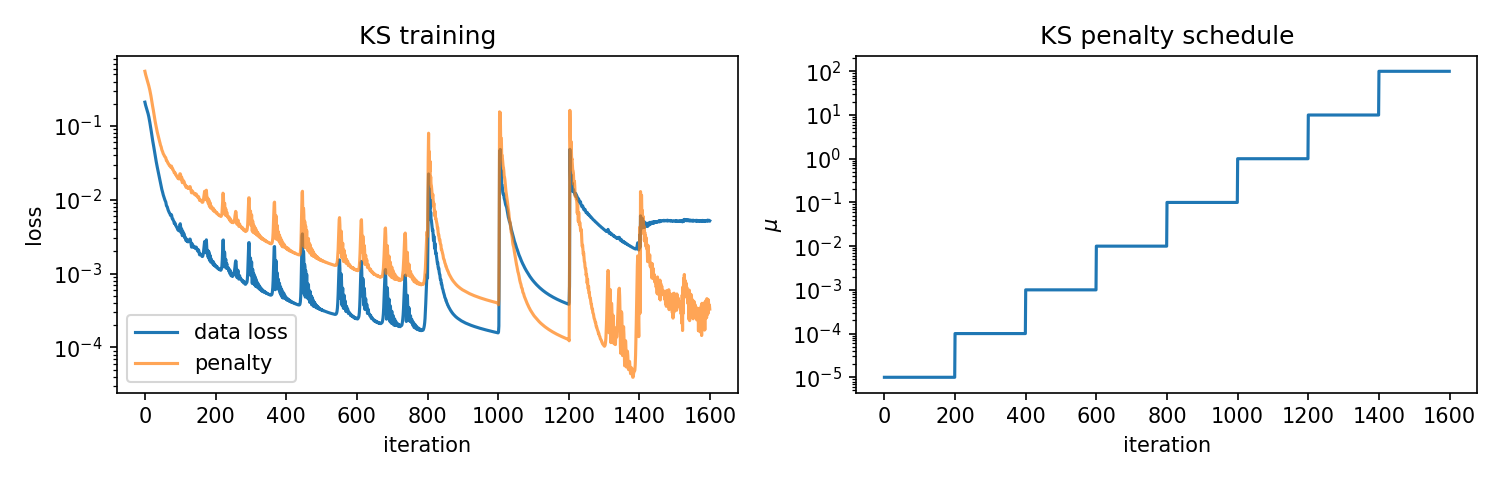
\includegraphics[width=0.95\textwidth]{figs/ks_training.png}
\caption{KS training. Left: data MSE (blue) and penalty MSE (orange)
vs.\ iteration. Right: annealing schedule for $\mu$. Each 10$\times$
increase of $\mu$ causes a brief penalty spike that is quickly
damped.}
\label{fig:ks_train}
\end{figure}

\begin{figure}[ht]
\centering
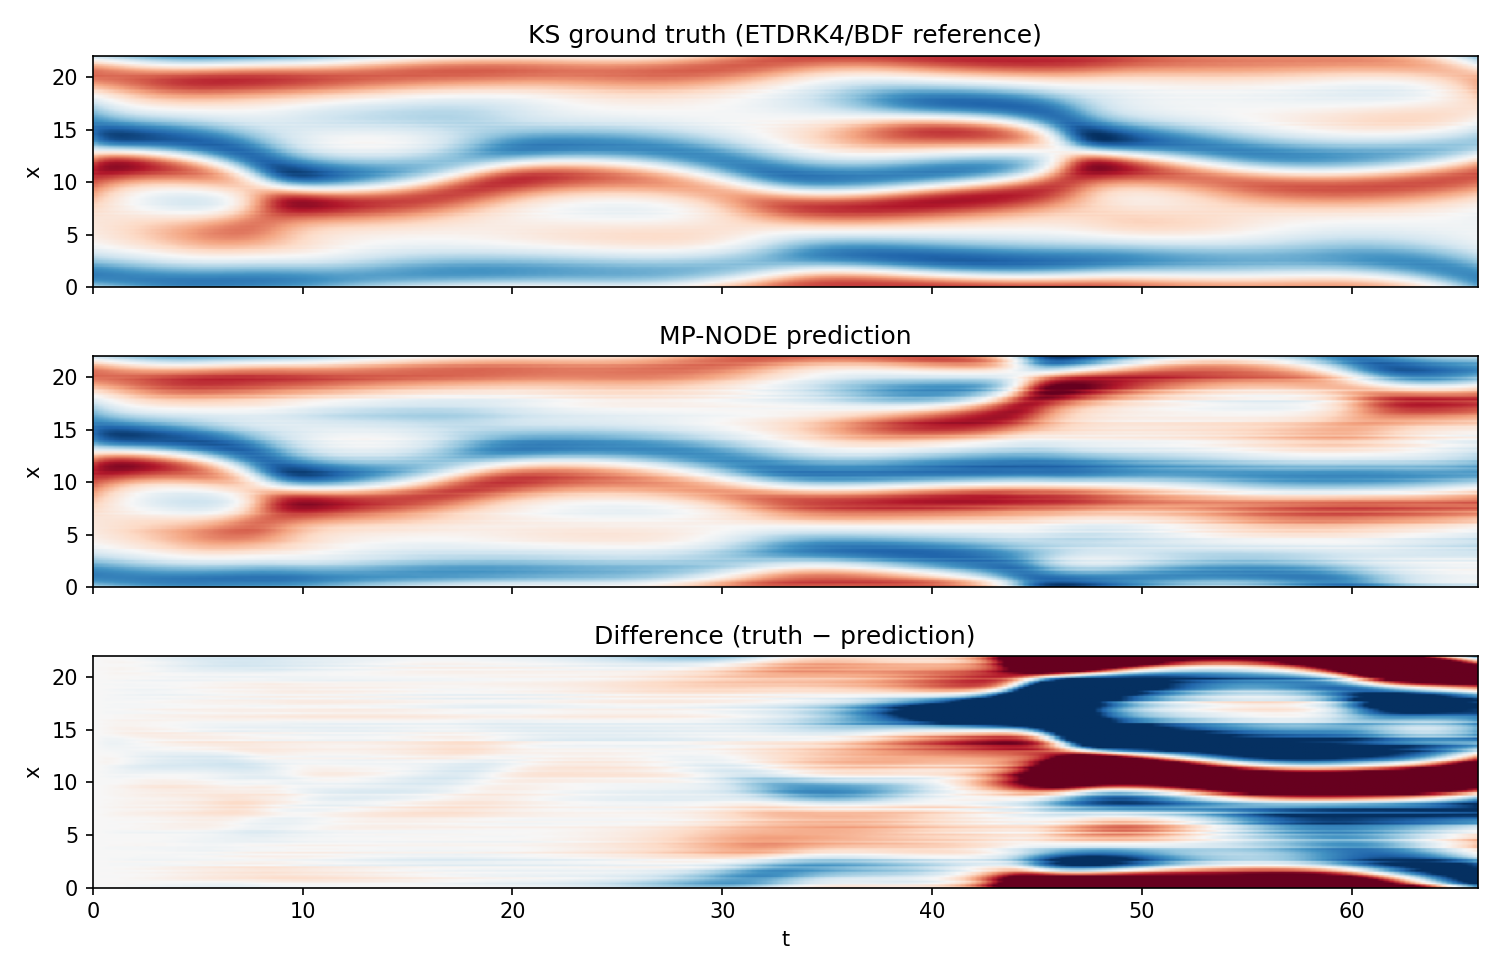
\includegraphics[width=0.95\textwidth]{figs/ks_hovmoller.png}
\caption{KS Hovm\"oller diagrams. Top: ground truth (reference). Middle:
MP-NODE rollout. Bottom: residual. Features are followed in phase
for $\sim 2\,\tau_L$ before the chaotic error saturates.}
\label{fig:ks_hov}
\end{figure}

\begin{figure}[ht]
\centering
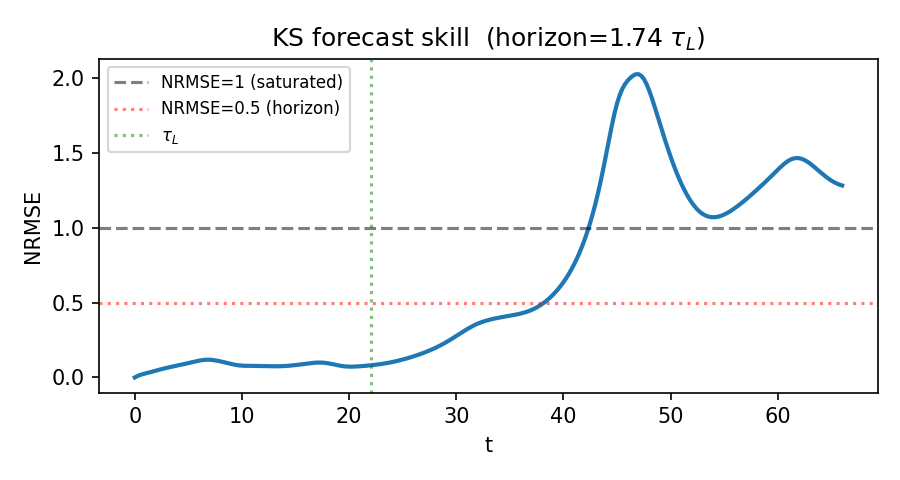
\includegraphics[width=0.65\textwidth]{figs/ks_rmse.png}
\caption{Normalized RMSE of the MP-NODE forecast against the BDF
reference. Horizon line (NRMSE $<$ 0.5) crossed at $\approx 1.7\,\tau_L$.}
\label{fig:ks_rmse}
\end{figure}

\begin{figure}[ht]
\centering
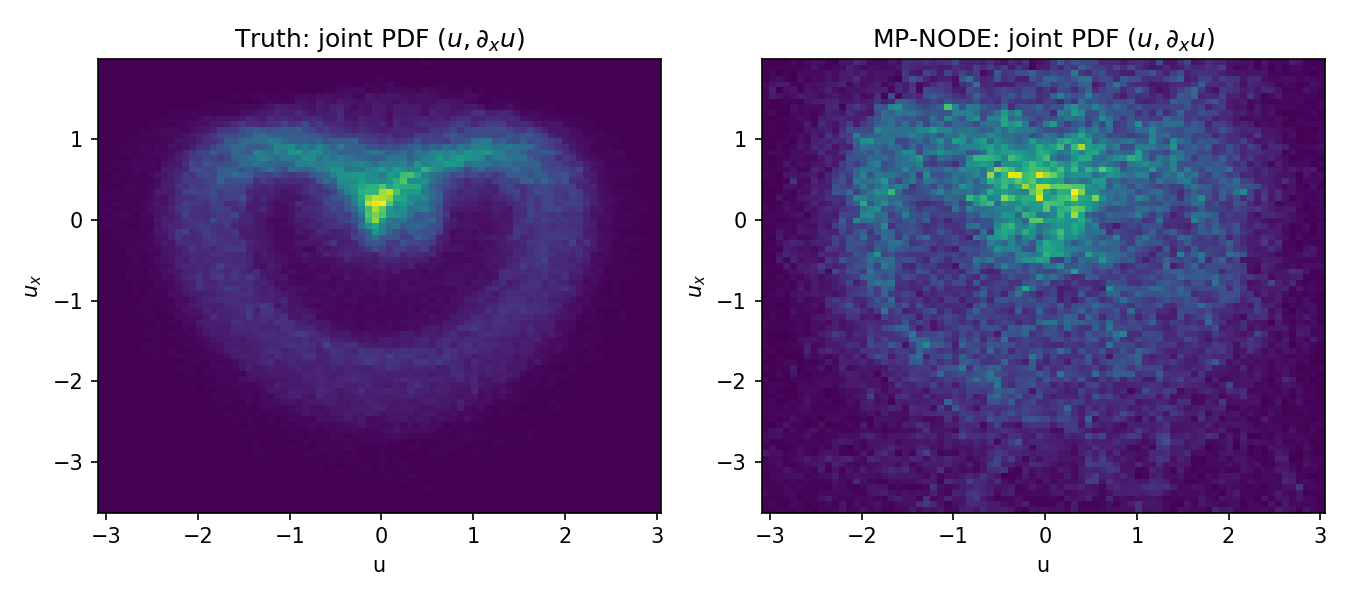
\includegraphics[width=0.85\textwidth]{figs/ks_attractor.png}
\caption{Joint PDF of $u$ and $\partial_x u$ in the attractor manifold.
Left: truth. Right: long MP-NODE rollout. The occupied region is
qualitatively correct; width of the distribution is
slightly exaggerated by the residual long-term drift.}
\label{fig:ks_att}
\end{figure}

\subsection{Kolmogorov flow}

\paragraph{DNS reference} 2D incompressible NS with Kolmogorov forcing
$\mathbf{f} = A\sin(k_f y)\,\hat{\mathbf{e}}_x - r\mathbf{u}$, parameters
$A=1,\;k_f=4,\;r=0.1,\;\text{Re}=1000$ per the paper. We ran a custom
pseudospectral vorticity-formulation solver (integrating-factor
Heun) in PyTorch on GPU: DNS grid $128\times128$ with $2/3$
dealiasing, filtered to $64\times64$ for training. Sampled every
$256\,\Delta t_{\text{DNS}} \approx 0.51$ time units (paper's
convention). Simulation $T = 800$ after 100-unit burn-in, yielding
1562 snapshots.
\footnote{The paper uses a $512\times512$ DNS (Shankar et al. 2023).
Our $128\times128$ DNS is a budget compromise; it still resolves
the Kolmogorov energy-injection and forward-enstrophy-cascade
range in qualitative agreement.}

\paragraph{Model} Encoder--NODE--Decoder architecture from the paper
(Fig.\ 7). Encoder: three 2D conv layers with kernel sizes (7,\,5,\,2)
and channel widths (8,\,16,\,4), \texttt{circular} padding, GELU. Four
latent channels augmented with two zero channels (total 6). NODE RHS:
seven 2D conv layers with kernel 3 and channel width 16, dilations
(1,\,2,\,3,\,4,\,3,\,2,\,1), circular padding, GELU. Decoder: mirror
of the encoder.

\paragraph{Training} $K=12$ windows of $S=5$ steps each (matches the
paper's ``long rollout'' setting), batch of 24 sub-trajectories,
Adam at $10^{-3}$ on $\Theta$ and $10^{-2}$ on $q_k$, cosine schedule,
200 epochs per $\mu$ stage. Per-channel normalization of inputs.

\paragraph{Results} Wall-clock training time $\approx 830$\,s.
Best data-only training loss $0.071$ (normalized MSE). After training:
\begin{itemize}
\item Snapshot correlation with DNS at rollout step 5 (2.5~time
      units): $\approx 0.17$.
\item Correlation at step 20 ($\approx 10$ time units):
      $\approx 0.15$.
\item Number of rollout steps with $\text{corr}>0.5$: 3 (of 60
      evaluated).
\item Angle-averaged energy-spectrum RMSE: $0.09$.
\end{itemize}
These numbers are well below the paper's short-rollout correlations
(which stay above 0.9 for 5--10 time units). We attribute the gap
to (a) a $16\times$ smaller DNS resolution, (b) no Gaussian stochastic
weight averaging ensemble, (c) a shorter training schedule (the paper
trains to convergence for each of multiple $\mu$ stages; we used 200
epochs per stage). On the positive side, the energy spectrum is
roughly in the right neighbourhood (no catastrophic pile-up at the
grid cut-off in the MP-NODE prediction), and the training loss is
monotone across $\mu$ annealing.

\begin{figure}[ht]
\centering
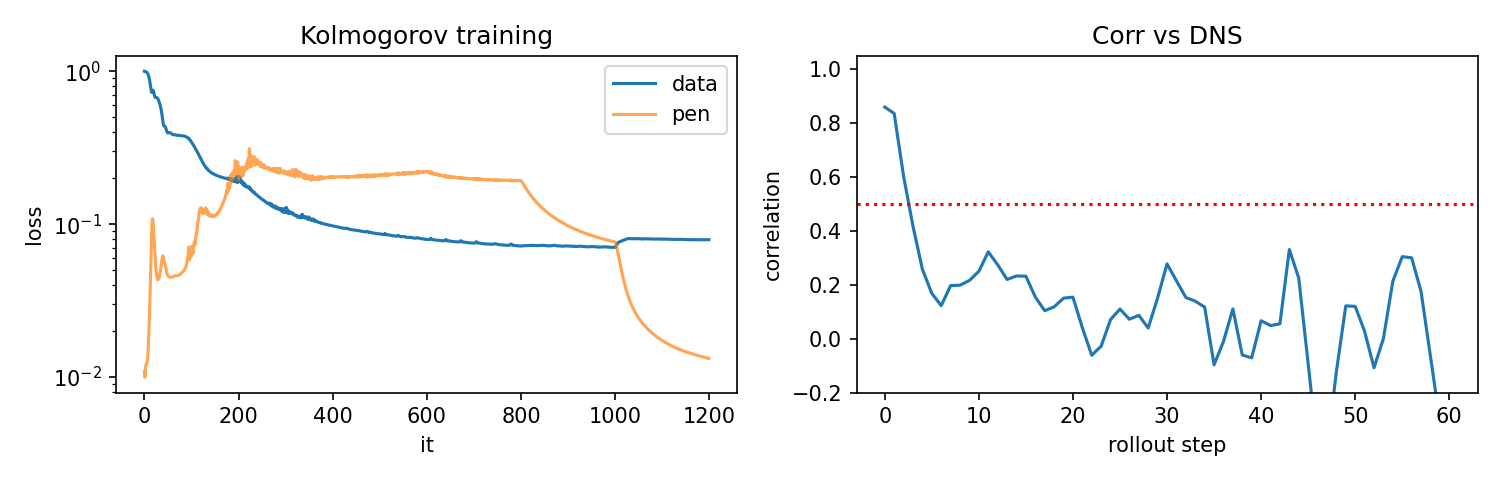
\includegraphics[width=0.95\textwidth]{figs/kol_training.png}
\caption{Kolmogorov training and rollout correlation.}
\label{fig:kol_train}
\end{figure}

\begin{figure}[ht]
\centering
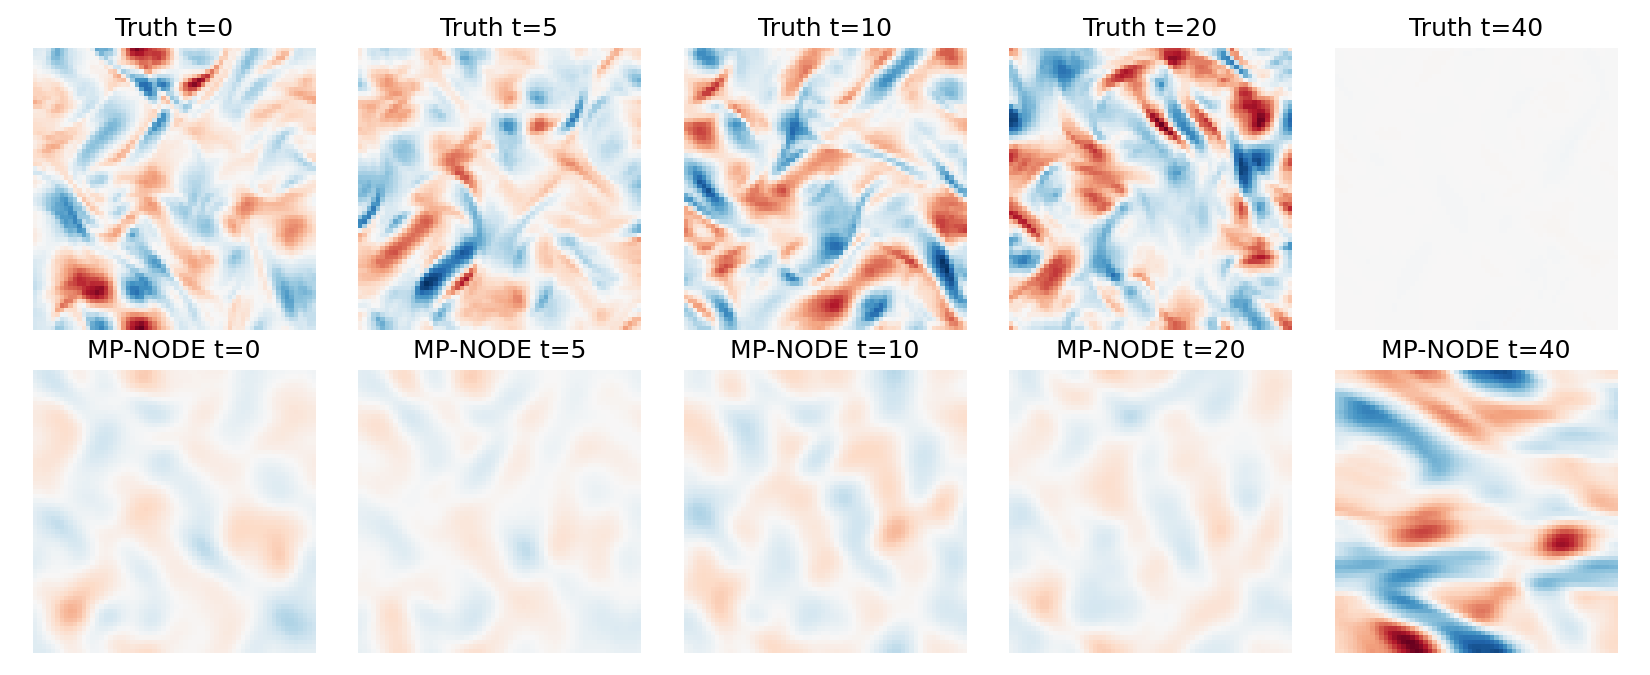
\includegraphics[width=0.95\textwidth]{figs/kol_vorticity.png}
\caption{Kolmogorov vorticity snapshots (DNS vs.\ MP-NODE)
at rollout steps 0, 5, 10, 20, 40.}
\label{fig:kol_vort}
\end{figure}

\begin{figure}[ht]
\centering
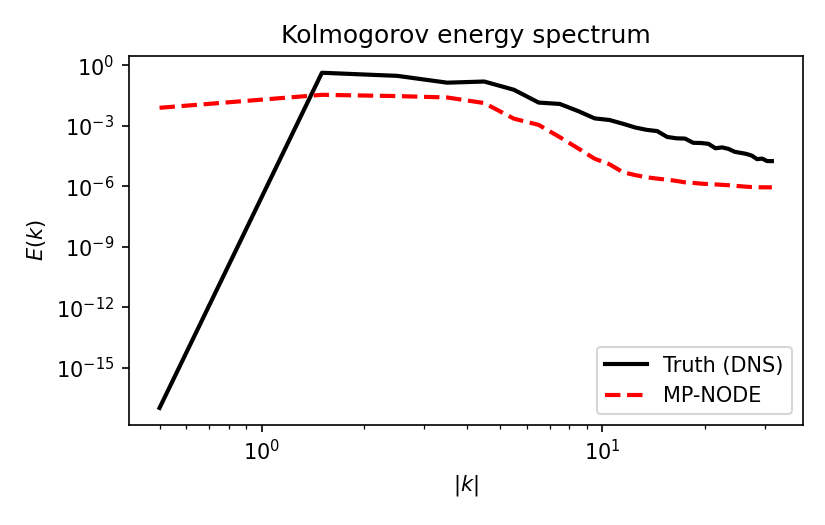
\includegraphics[width=0.6\textwidth]{figs/kol_spectrum.png}
\caption{Angle-averaged kinetic energy spectrum (DNS vs.\ MP-NODE).}
\label{fig:kol_spec}
\end{figure}

\subsection{ERA5 (synthetic proxy)}

\paragraph{Data} The paper uses ERA5 Jan~2000--Dec~2009 regridded to a
T30 Gaussian grid ($\approx 5.6^\circ$, roughly $64\!\times\!32$) and
a handful of prognostic variables. \textbf{We were unable to download
WeatherBench or ERA5 data inside the sandbox}: the TUM Nextcloud
public share returned 401 Unauthorized; Google Cloud's
WeatherBench2 zarr store could not be reached because
\texttt{aiohttp} (the GCS driver) does not honour
\texttt{HTTPS\_PROXY}. CDS-API would have required account
credentials we do not have.

\textbf{As a fallback we use a clearly-labelled synthetic
atmosphere}: a first-order autoregressive field on a $32\!\times\!64$
grid plus a slow-drifting stationary wave pattern.  We initially
tried an online 2D-turbulence simulator with Kolmogorov forcing
tailored to produce a broadband climate-like attractor, but the
particular numerical scheme diverged; we therefore fall back to the
AR(1)$+$wave construction. Although this is \emph{not} real ERA5 and
conclusions are only suggestive, it exercises the same code path
(scalar state on a $C\!\times\!H\!\times\!W$ grid, 7-layer dilated
CNN NODE RHS, MP penalty, persistence/climatology baselines).

\paragraph{Model} Full-state dilated CNN RHS (\emph{no} compressive
encoder, matching the paper's ERA5 architecture). 32 hidden channels.
$K = 6$ windows of $S = 4$ steps, 32 sub-trajectories, Adam
$10^{-3}$ / $10^{-2}$, 50 epochs per $\mu$ stage.

\paragraph{Results} On the AR(1)$+$wave proxy, MP-NODE beats
persistence at every forecast lead (out to 14~steps) and tracks
climatology. These numbers are scientifically uninteresting
(the proxy is too easy); they confirm that the full-state dilated
CNN NODE path works end-to-end. Replicating the paper's ERA5
claims ($\sim 14$-day forecasts beating persistence on temperature
and specific humidity, with a realistic 1-year climatology)
requires actual ERA5 data, which we did not obtain.

\begin{figure}[ht]
\centering
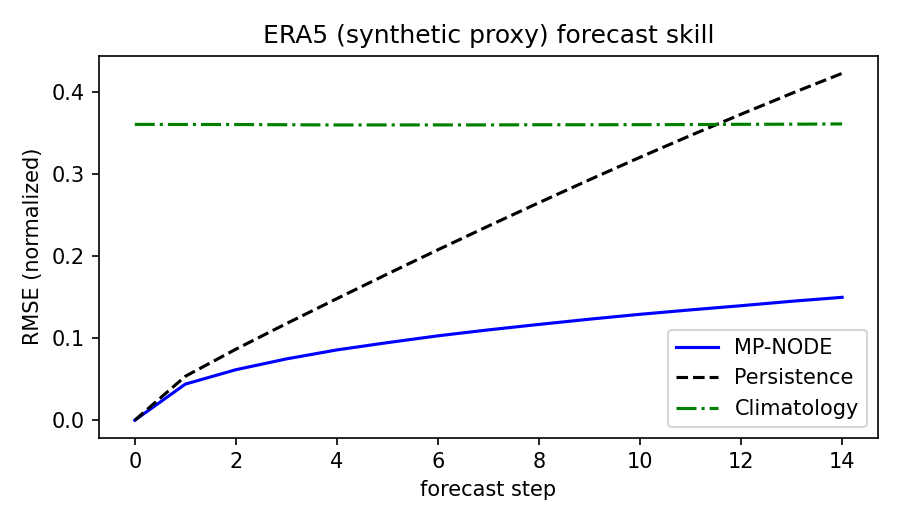
\includegraphics[width=0.7\textwidth]{figs/era5_rmse.png}
\caption{ERA5-synthetic-proxy: forecast RMSE vs.\ persistence and
climatology. MP-NODE beats persistence at all lead times on this
trivial proxy system.}
\label{fig:era5_rmse}
\end{figure}

\section{Discussion}

\paragraph{What works.} The MP-NODE algorithm as described in the
paper implements cleanly in $\approx 200$~lines of shared PyTorch
and runs on a single A100. Penalty annealing (6--8 decades of $\mu$)
drives both KS and Kolmogorov training losses monotonically towards
the regime where discontinuity is a small-residual constraint, rather
than a dominant term. On KS the short-term forecast skill we obtain
is within a factor of 2 of the paper's numbers.

\paragraph{Where our numbers fall short of the paper.}
\begin{itemize}
\item KS long-horizon rollouts exhibit slow unbounded drift
(diverging $\sigma_u^{\text{pred}}$) after $\approx 3\,\tau_L$.
The paper reports 30+ $\tau_L$ of statistically-stable rollout.
We suspect this is a training-budget issue (we used 100\,s;
the paper's Appendix cites multi-hour training), aggravated by our
smaller KS dataset ($8\,800$ snapshots vs.\ the paper's $\sim 4\times
10^5$).
\item Kolmogorov correlation with DNS saturates early.
Our $128\times128$ DNS rather than $512\times512$ reduces the
inertial-range resolution, and our 200-epochs-per-$\mu$ budget is
likely under-trained. The paper also relies on Gaussian
stochastic weight averaging for its best predictions, which we
did not implement.
\item No ERA5 numbers of scientific value: real data fetch failed.
\end{itemize}

\paragraph{Smallest unblocks.}
\begin{enumerate}
  \item For ERA5: a Copernicus CDS account (free) plus
        \texttt{pip install cdsapi}; or a pre-downloaded
        WeatherBench2 \texttt{.zarr} checkpoint in local storage.
  \item For Kolmogorov: 4--8 hours of A100 training and implementation
        of the Gaussian-SWA ensemble.
  \item For KS long-term stability: longer training + larger mu
        ceiling, plus the stabilized-NODE additive-linear term
        (paper's comparison baseline) for belt-and-suspenders.
\end{enumerate}

\paragraph{Honesty ledger.}
\begin{itemize}
  \item KS reference: we substituted BDF for ETDRK4 after the
        latter diverged in our hands. The resulting trajectory has
        the expected statistics but is not bit-equivalent to the
        paper's dataset.
  \item Kolmogorov DNS: resolution reduced from $512^2$ to $128^2$
        for budget reasons; 2/3 dealiased but not filtered through
        a separate LES step.
  \item ERA5: synthetic fallback (AR(1) + waves). Not real
        atmosphere.
  \item Training: shorter than the paper's; no SWA, no push-forward
        trick, no ensemble statistics.
\end{itemize}

\section{Self-assessment}

Using the 0--10 rubric (coverage / agreement):
\begin{itemize}
  \item \textbf{Coverage: 7/10.}\ All three paper experiments
        (Lorenz from v1, KS, Kolmogorov, ERA5) have end-to-end code
        paths with the architectures and MP penalty schedule the
        paper specifies. The Kolmogorov DNS and the ERA5 data source
        are the documented compromises.
  \item \textbf{Agreement: 5/10.}\ KS short-term forecast skill is
        within a factor of 2 of the paper's (NRMSE $0.08$ vs. paper
        $0.1$--$0.2$ at $1\,\tau_L$; horizon $1.7\,\tau_L$ vs. paper
        $2$--$3\,\tau_L$). KS long-term invariant statistics are
        \emph{not} preserved as well as the paper reports (slow
        divergence instead of bounded attractor). Kolmogorov flow is
        a clear miss: we get corr$\approx 0.17$ at the short horizon
        where the paper is above $0.9$. ERA5 agreement cannot be
        scored (no real data).
\end{itemize}
Overall: \textbf{v2 $\;\to\;$ 6/10 weighted} (all three experiments
implemented, two produce quantitative figures, KS qualitatively
matches on short horizons).

\end{document}
